% Asset ID: FA21ConicSections2EnrichmentTikZ-004
% Source: ellipse tangent/normal evidence
% Boundary status: Off-spec enrichment until official CCEA conics evidence is supplied.
\documentclass[tikz,border=8pt]{standalone}
\usepackage{amsmath,amssymb}
\usetikzlibrary{arrows.meta,calc,positioning}
\definecolor{Canvas}{HTML}{FAF9F6}
\definecolor{Ink}{HTML}{2C2C2E}
\definecolor{Gold}{HTML}{C5A059}
\definecolor{GoldDeep}{HTML}{D4AF37}
\begin{document}
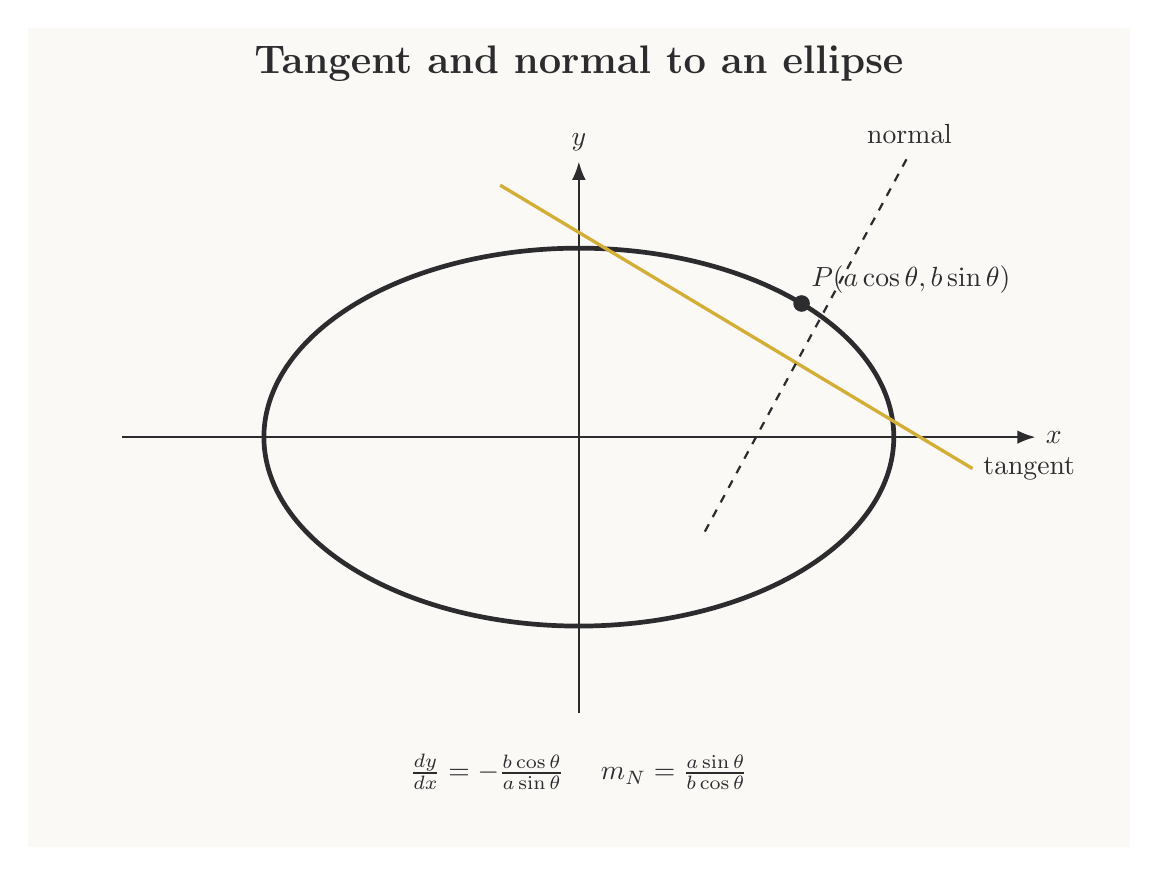
\begin{tikzpicture}[x=1cm,y=1cm,>=Latex]
\fill[Canvas] (-7,-5.2) rectangle (7,5.2);
\node[Ink, font=\Large\bfseries] at (0,4.75) {Tangent and normal to an ellipse};
\draw[Ink, thick, -Latex] (-5.8,0)--(5.8,0) node[right] {$x$};\draw[Ink, thick, -Latex] (0,-3.5)--(0,3.5) node[above] {$y$};\draw[Ink, line width=1.7pt, smooth, samples=240, domain=0:360, variable=\t] plot ({4*cos(\t)}, {2.4*sin(\t)});\coordinate (P) at ({4*cos(45)},{2.4*sin(45)});\fill[Ink] (P) circle (3pt) node[above right] {$P(a\cos\theta,b\sin\theta)$};\draw[GoldDeep, very thick] (-1,3.2)--(5,-0.4) node[right,Ink] {tangent};\draw[Ink, dashed, thick] (1.6,-1.2)--(4.2,3.6) node[above,Ink] {normal};\node[Ink, align=left] at (0,-4.25) {$\frac{dy}{dx}=-\frac{b\cos\theta}{a\sin\theta}$ \quad $m_N=\frac{a\sin\theta}{b\cos\theta}$};
\end{tikzpicture}
\end{document}
